\documentclass{beamer}

\usepackage[utf8]{inputenc}
\usepackage[spanish]{babel}
\usepackage{amsmath}
\usepackage[nosetup]{evan}
%\usetheme{Goddard}
\usetheme{Madrid}
\hypersetup{colorlinks,allcolors=.,urlcolor=magenta}
\usepackage[table]{xcolor} % Para definir colores en tablas
\usepackage{graphicx} % Para redimensionar la tabla

\title{Métodos Numéricos}
\subtitle{Unidad 1: Teoría Elemental de Errores}
\author[Ricardo Largaespada]{Ricardo Jesús Largaespada Fernández}
\institute[UNI]{Ingeniería de Sistemas, DACTIC, UNI}
\date{03 de Marzo, 2025}

\usepackage{listings}
\usepackage{xcolor}

\lstset{
  language=Matlab,
  inputencoding=utf8,
  extendedchars=true,
  basicstyle=\ttfamily\footnotesize,
  keywordstyle=\color{blue},
  commentstyle=\color{green!50!black},
  stringstyle=\color{red},
  numbers=left,
  numberstyle=\tiny,
  stepnumber=1,
  numbersep=5pt,
  frame=single,
  backgroundcolor=\color{gray!10},
  captionpos=b,
  breaklines=true,
  literate=%
    {á}{{\'a}}1 {é}{{\'e}}1 {í}{{\'i}}1 {ó}{{\'o}}1 {ú}{{\'u}}1
    {Á}{{\'A}}1 {É}{{\'E}}1 {Í}{{\'I}}1 {Ó}{{\'O}}1 {Ú}{{\'U}}1
    {ñ}{{\~n}}1 {Ñ}{{\~N}}1
}

\begin{document}

\frame{\titlepage}

\begin{frame}
\frametitle{Agenda}
\tableofcontents
\end{frame}

\section{Datos Generales}
\begin{frame}
\frametitle{Datos del Curso}
\begin{itemize}
    \item \textbf{Asignatura}: Métodos Numéricos
    \item \textbf{Créditos}: 3
    \item \textbf{Frecuencia Semanal}: 3 sesiones
    \item \textbf{Semestre Académico}: Quinto Semestre (3er año)
    \item \textbf{Carrera}: Ingeniería de Sistemas
    \item \textbf{Horario de Atención}: Lu | Mi | J: 3M | 2M | 1M
    \item \textbf{Grupos}: 3M3-SIS-S
\end{itemize}
\end{frame}

\section{Objetivo General}
\begin{frame}
\frametitle{Objetivo General de la Asignatura}
\begin{itemize}
    \item Aproximar por métodos numéricos la solución de diferentes problemas de Ingeniería y Ciencias que no tienen solución analítica, diseñando el algoritmo adecuadamente y obteniendo la solución, mediante el uso de Calculadoras o  Software Matemáticos, de una forma rápida y efectiva.
\end{itemize}
\end{frame}

\section{Plan Temático}

\begin{frame}
\frametitle{Plan Temático}
\begin{center}
    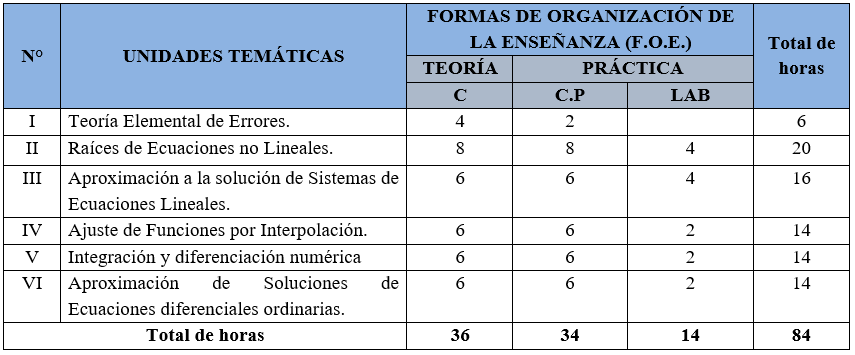
\includegraphics[scale=.5]{images/plan_tematico.png}
\end{center}
\end{frame}

\section{Unidad 1: Teoría Elemental de Errores}
\begin{frame}
\frametitle{Objetivos de Unidad 1}
    \begin{itemize}
        \item Identificar los distintos tipos de errores que se generan en el empleo de los métodos numéricos, desde el punto de vista de la aritmética flotante que evidencien en la realización de un determinado cálculo.
        \item Calcular los errores absolutos y relativos en redondeos con operaciones aritméticas obteniendo el valor más próximo a la operación realizada e interpretando la magnitud e influencia de estos errores.
        \item Aceptar que en la aritmética flotante los errores cometidos son inevitables tanto en los cálculos manuales, con calculadora y con computadora teniendo presente que en su trabajo profesional siempre deberá existir un margen de tolerancia en sus mediciones.
    \end{itemize}
\end{frame}

\begin{frame}{Únete al Grupo de WhatsApp}
    \centering
    Para facilitar la comunicación del curso, únete al grupo de WhatsApp escaneando el siguiente código QR o haciendo clic en el enlace:  

    \vspace{0.5cm}
    
    
\includegraphics[width=4cm]{images/whatsapp_mn2025.png} % Reemplaza con tu archivo QR
    
    \vspace{0.5cm}

    \Large \textbf{\href{https://chat.whatsapp.com/Liee39TzC9U0Q9u5E0f5Ff}{Únete aquí al grupo}}
    
    \vspace{0.5cm}

    ¡No olvides presentarte al ingresar!
\end{frame}

\begin{frame}{Acceso a Licencia Académica de MATLAB}
    \centering
    Para acceder a la versión académica de MATLAB, usa el siguiente enlace:  
    \vspace{0.5cm}
    \begin{center}

\includegraphics[width=4cm]{images/matlab_license.png}
    \end{center}
    \Large \textbf{\href{https://www.mathworks.com/licensecenter/classroom/laff/}{MathWorks License Center}}  
    
    \vspace{0.5cm}
    
    Esta licencia está diseñada para entornos de aprendizaje y permite el uso de MATLAB en el aula y en proyectos académicos.
\end{frame}

\section{Sesión 1}
\begin{frame}
\frametitle{Sesión 1}

\textbf{Tema}
\begin{enumerate}
\item Necesidad de los Métodos Numéricos.
\item Aproximaciones y Errores.
\begin{enumerate}
\item Redondeo. Tipos de Redondeo.
\end{enumerate}
\end{enumerate}
\textbf{Objetivo}
\begin{itemize}
    \item El estudiante identificará la necesidad de los métodos numéricos y comprenderá los conceptos de aproximaciones, errores y tipos de redondeo, incluyendo el epsilon de máquina, mediante una conferencia interactiva y ejemplos prácticos básicos.
\end{itemize}
\end{frame}

% Pregunta inicial
\begin{frame}
    \centering
    \Large ¿Qué son los métodos numéricos?
    \\[1cm]
    ¿En qué situaciones reales podríamos necesitarlos?
\end{frame}

\begin{frame}{Caso Real: Cálculo de Intereses en Sistemas Bancarios}
    \begin{columns}
        \column{0.6\textwidth}
        En los sistemas bancarios, los algoritmos numéricos se utilizan para calcular los intereses generados en cuentas de ahorro y créditos.  
        
        \textbf{Pregunta:} ¿Cómo afectaría un error numérico en estos cálculos?  
        
        - ¿Podría un banco cobrar más o menos intereses debido a un error en la precisión?  
        - ¿Cómo influyen los métodos de redondeo en la facturación y los estados de cuenta?  
        
        Estos cálculos dependen de \textbf{métodos numéricos} para la integración de tasas de interés y redondeo en las transacciones.

        \column{0.4\textwidth}
        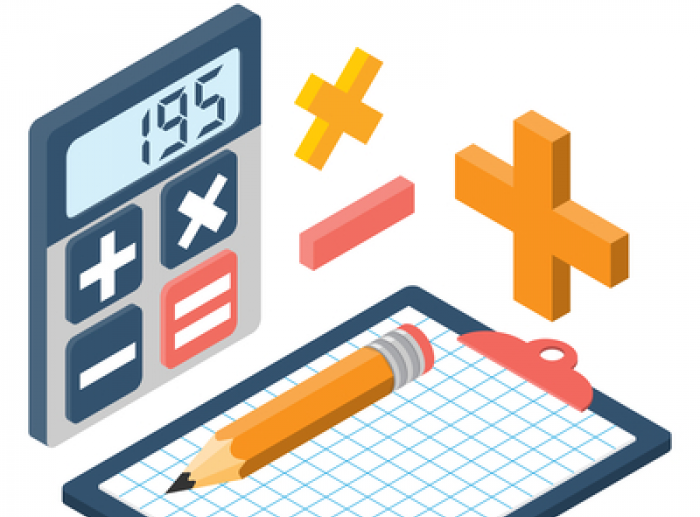
\includegraphics[width=\textwidth]{images/calculo_intereses.png} % Imagen representativa
    \end{columns}
\end{frame}

% Comparación de soluciones
\begin{frame}{Soluciones Analíticas vs. Soluciones Numéricas}
    \begin{columns}
        \column{0.5\textwidth}
        \textbf{Soluciones Analíticas}
        \begin{itemize}
            \item Basadas en ecuaciones exactas.
            \item No dependen de aproximaciones.
            \item Ejemplo: Resolver $x^2 - 4 = 0$ tiene solución exacta $x = \pm2$.
        \end{itemize}
        
        \column{0.5\textwidth}
        \textbf{Soluciones Numéricas}
        \begin{itemize}
            \item Basadas en métodos aproximados.
            \item Necesarias cuando no hay solución cerrada.
            \item Ejemplo: Resolver $e^x - x^2 = 0$ mediante un método iterativo.
        \end{itemize}
    \end{columns}
\end{frame}

% Tipos de errores con ejemplos visuales
\begin{frame}{Errores en los Cálculos}
    \begin{itemize}
        \item \textbf{Error Absoluto}: Diferencia entre el valor exacto y el valor aproximado.
        \item \textbf{Error Relativo}: Proporción del error absoluto respecto al valor exacto.
        \item \textbf{Error de Redondeo}: Ocurre cuando se trunca un número decimal.
    \end{itemize}
    \centering
    %\includegraphics[width=0.7\textwidth]{error_redondeo.jpg} % Imagen de error de redondeo
\end{frame}

% Pregunta antes de epsilon de máquina
\begin{frame}
    \centering
    \Large ¿Cuán precisos son los cálculos en una computadora?
\end{frame}

\begin{frame}{Epsilon de Máquina}
    \textbf{Definición:} Es el número positivo más pequeño que, sumado a 1, produce un resultado diferente de 1 en una computadora.

    \vspace{0.5cm} % Espaciado antes del código para evitar problemas de compilación

    \textbf{Código en MATLAB:}
    
\lstinputlisting[language=Matlab, frame=single, caption={Cálculo del Epsilon de Máquina en MATLAB}]{codes/epsilon_maquina.m}
    
    \vspace{0.5cm} % Espaciado después del código para mejorar la presentación
\end{frame}


\end{document}
